\documentclass[10pt, a4paper, sigplan, authordraft]{acmart}
% authordraft

\title{On the Relevance of Type Analysis of Low-level Code}

\author{Robin Eklind}
\affiliation{
	\institution{Royal Institute of Technology (KTH)}
	\city{Stockholm}
	\country{Sweden}
}
\orcid{0000-0003-0275-5514}

\keywords{type analysis, type recovery, type inference, type lattice, type constraints, decompilation, reverse engineering, low-level code, assembly, LLVM IR, SSA, formal verification, binary analysis, static analysis}

% skip headers
\pagestyle{plain}

% skip copyright notice
\setcopyright{none}
% printacmref (skip ACM reference format)
% printfolios (print page numbers)
\settopmatter{printacmref=false,printfolios=true}

% remove conference information in footnote.
\renewcommand\footnotetextcopyrightpermission[1]{}

% skip DOI
\acmDOI{}

% skip ISBN
%\acmISBN{012-3-456-78933-3 (fake)}
\acmISBN{}

% Conference - fake
\acmConference[POPL'19]{ACM Conference}{January 2019}{Lisbon, Portugal (fake)}
\acmPrice{0.00}

% use ACM bibliography style
\bibliographystyle{ACM-Reference-Format}

\begin{document}

% === [ Front matter ] =========================================================

% --- [ Abstract ] -------------------------------------------------------------

% TODO: Remove abstract?

%\begin{abstract}
%foo
%\end{abstract}

% --- [ Teaser image ] ---------------------------------------------------------

\begin{teaserfigure}
	\centering
	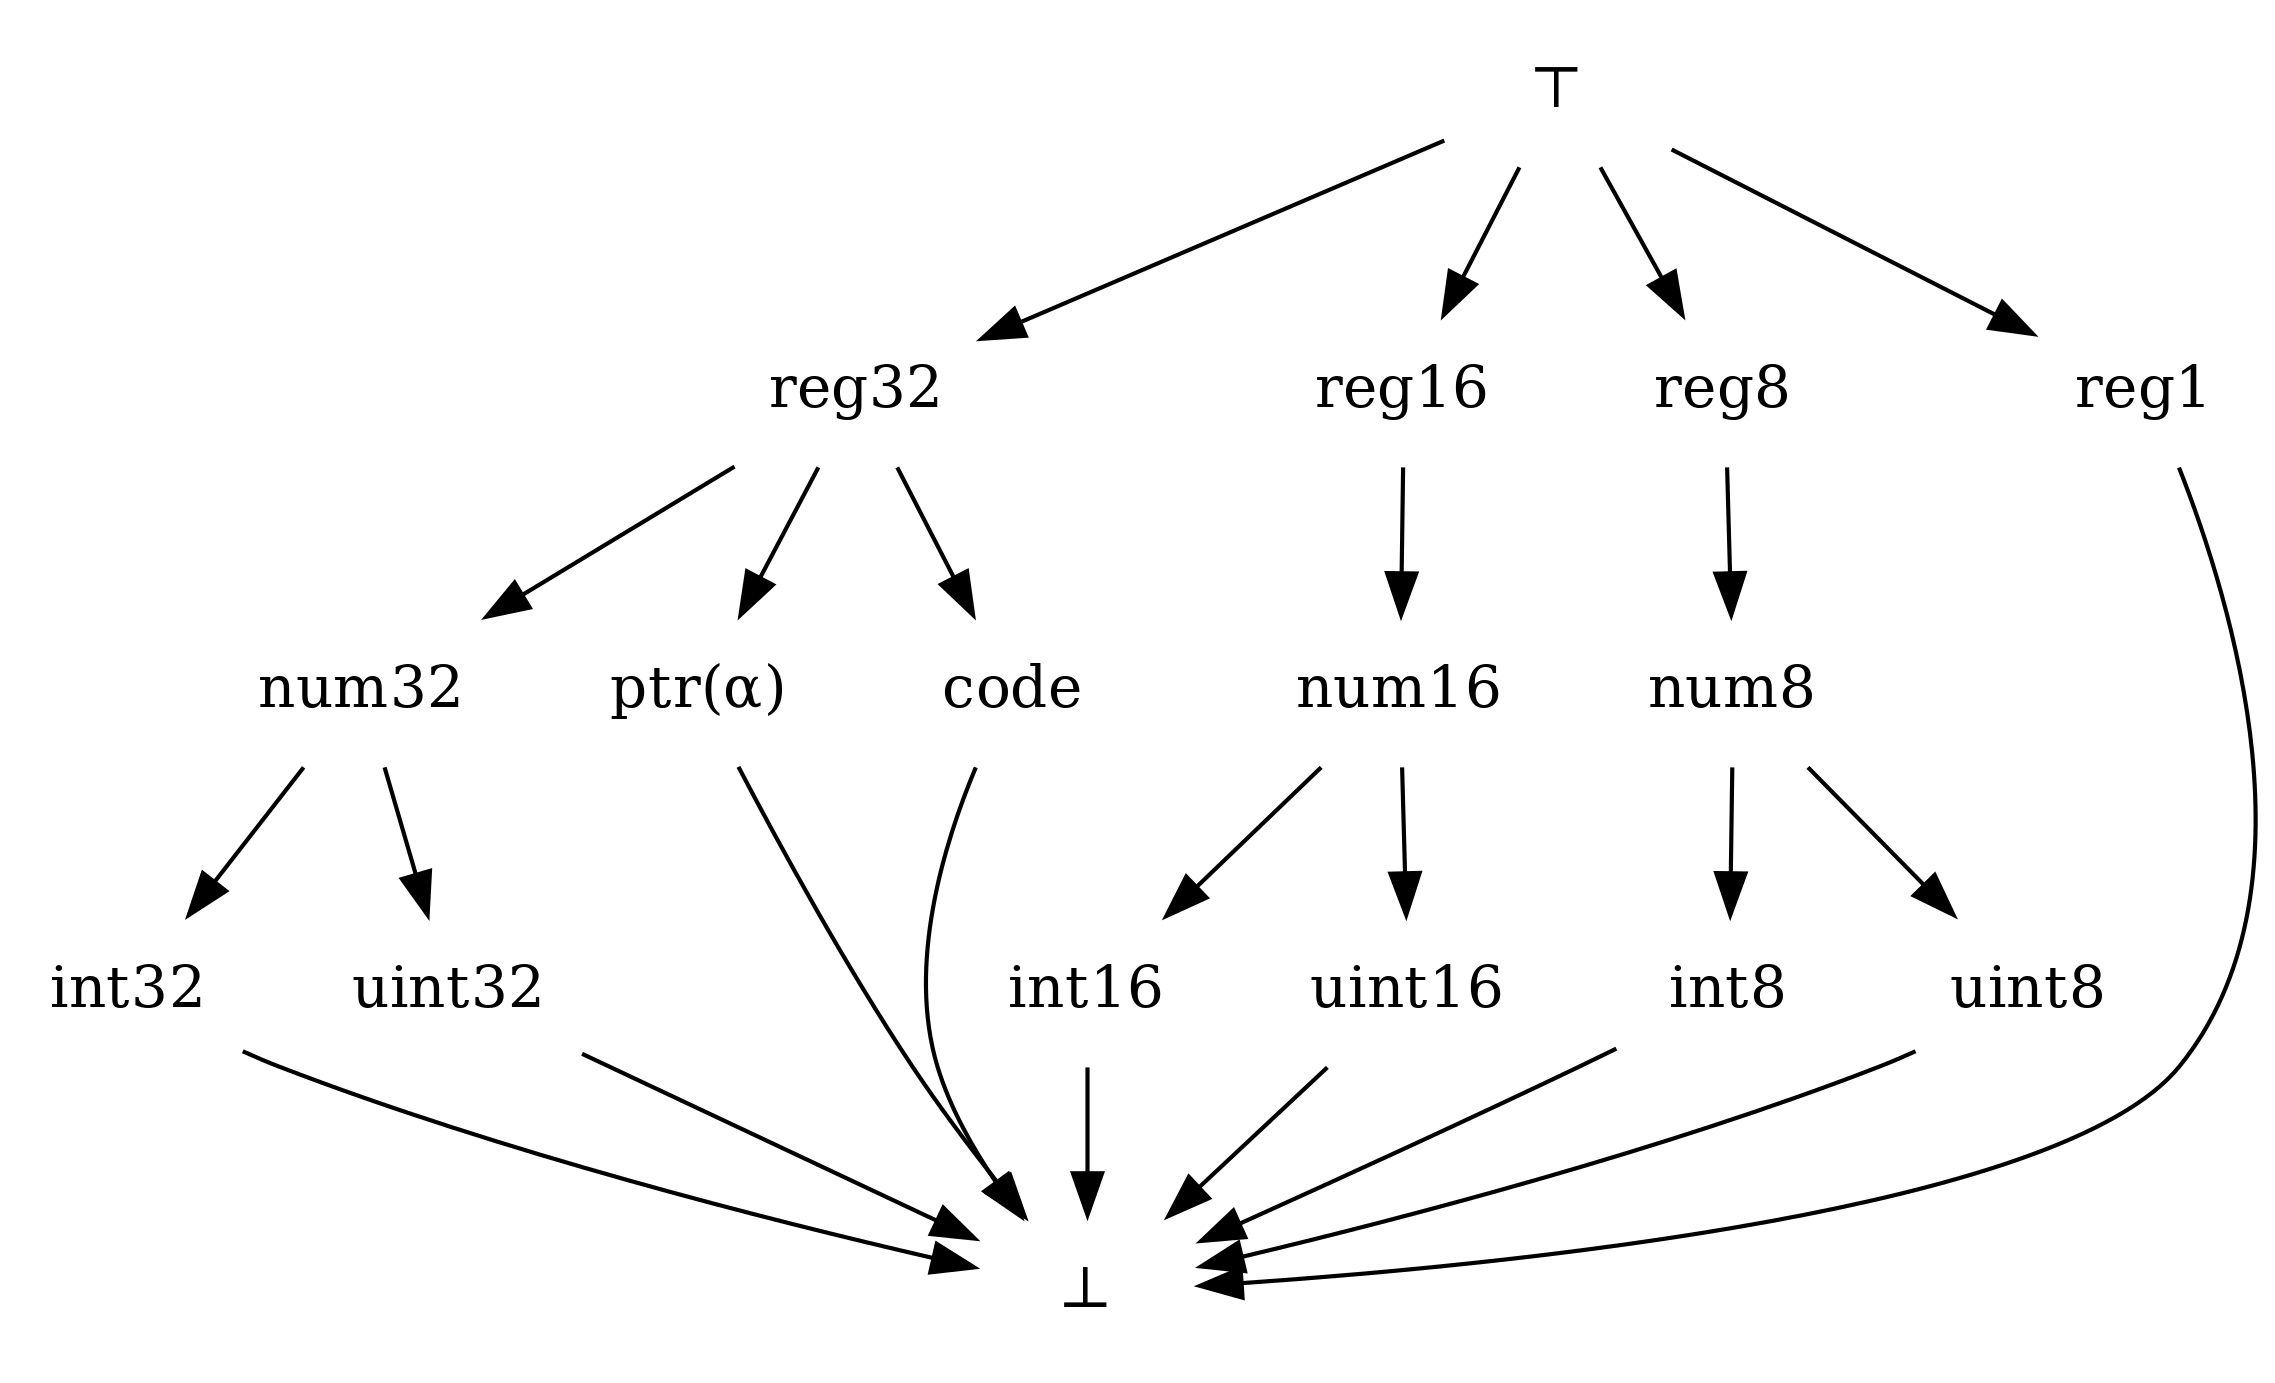
\includegraphics[width=0.5\textwidth]{inc/base_type_lattice.png}
	\caption{Primitive type lattice of TIE}
	\label{fig:base_type_lattice}
\end{teaserfigure}

% --- [ Title ] ----------------------------------------------------------------

\maketitle

% === [ Main matter ] ==========================================================

% --- [ Introduction ] ---------------------------------------------------------

\section{Introduction}

% What is the problem to solve, and why is it important?
% - applications?

Take for a moment the opportunity to reflect on the magnitude at which we rely on the \textit{correct implementation} of software to provide the most vital infrastructure of society. With increasingly interconnected and interdependent systems -- often in polyglot environments -- faults may have far reaching real-world consequences. Implementation correctness may be validated through formal verification and static analysis of source code to proactively prevent entire categories of security vulnerabilities and limit the occurrence of bugs. However, frameworks for validation of source code are often tied to a specific source language or small set of languages (e.g. ADA and SPARK) and therefore have limited effectiveness in polyglot projects. Furthermore, inconsistent interpretation of source code between static analysis tools and compilers may lead to run-time errors even when statically proven never to occur \cite{ada_static_analysis_and_compiler_inconsistencies}. Finally, as demonstrated in Ken Thompson's 1984 Turing aware lecture \textit{Reflections on Trusting Trust}, the output of a compiler may not be trusted even if its input is formally verified, as the compiler environment may have been tampered\footnote{Not only theoretically, tempered environments is a real-world issue that large corporations such as Ericsson and Saab of Sweden have to deal with on a daily basis.} with:

\begin{quote}
	\textit{``No amount of source-level verification or scrutiny will protect you from using untrusted code.''} \cite{trusting_trust}
\end{quote}

For these reasons, conducting formal verification and semantic analysis on the output rather than the input of a compiler is relevant. To facilitate formal verification efforts and enable rich static analysis of binary executables, type analysis of low-level code (e.g. assembly) is essential as type information is lost during the process of compilation.

% Research question: is type analysis of low-level code a solved problem?

The aim of this meta study is to assess the state of research

% binary analysis,

% floating-point stack
%    - track stack top (indirect calls/external calls)
% pointer analysis
%    - global memory region
%    - stack memory region
%    - heap memory region
% registers
%    - live ranges; SSA
% structures/arrays

\paragraph{Scope}

% TODO: rephrase with cite's.

In scope foo and out of scope bar.

% --- [ Method ] ---------------------------------------------------------------

\section{Method}

A meta-study has been conducted to assess the body of research related to type recovery of low-level code.

% --- [ Results ] --------------------------------------------------------------

\section{Results}

foo

% --- [ Discussion ] -----------------------------------------------------------

\section{Discussion}

foo

% TODO: Move into appropriate sections.

% --- [ other] -----------------------------------------------------------

\section{Background}

foo

\paragraph{Static Single Assignment}

foo

% describe PHI instructions.

\section{Variable Recovery}

\paragraph{Value Set Analysis}

foo

upper bound, lower bound and stride for memory locations.

\paragraph{Function signature recovery}

The following set of steps are used for function signature recovery (function parameters and returns arguments) in SecondWrite \cite{scalable_type_detection}.

\begin{enumerate}
	\item assume all registers are arguments and no register are return arguments.
	\item registers written to are potential return arguments.
	\item callee saved registers (through push in function prologue and pop in function epilogue) (\textit{DeadStores}) are pruned from potential return set.
	\item prune arguments not actually used (e.g. not part of \textit{DeadStore} or PHI instructions).
	\item prune return registers not actually used by callers.
\end{enumerate}

\section{Type Recovery}

\paragraph{Type inference}

foo

\paragraph{Algorithm W}

foo

\paragraph{Unification}

foo

TODO: Describe the unification step, as many algorithms rely on this to discover struct types, etc.

\paragraph{Type lattice}

foo

Top type ($\top$): any type.

Bottom type ($\bot$): inconsistent type.

\paragraph{Pointer analysis}

foo

\paragraph{Type sink}

% TODO: rephrase.

Type can be resolved directly and is known to be correct. For instance, derived from function signatures of standard libraries.

\paragraph{Type revealing instruction}

foo

% TODO: rephrase.

Infer that the operand is of integer type, memory, floating-point, etc.


\paragraph{Type propagation}

foo

% Type constraints

\section{Evaluation}

foo

% using debug information

% evaluation metric

\paragraph{SPEC2006}


Type inference: type assignment algorithm W: \cite{milner_algorithmw}.

Type-based decompilation: \cite{mycroft_type_based_decompilation}.

%Comparison of type-based and proof-directed decompilation: \cite{mycroft_comparing_type_based_and_proof_directed_decompilation}

foo \cite{reverse_engineering_of_types}

foo \cite{scalable_type_detection}

foo \cite{bintype}

foo \cite{type_inference_on_executables}

foo \cite{dynstruct}

foo \cite{polymorphic_type_inference_for_machine_code}

% === [ Back matter ] ==========================================================

% --- [ References ] -----------------------------------------------------------

\clearpage

foo

\clearpage

\bibliography{references}

%\appendix
%\section{Appendix}
%
%foo

\end{document}
